\documentclass[12pt]{article}

% Packages
\usepackage{amsmath}
\usepackage{amssymb}
\usepackage{hyperref}
\usepackage{booktabs}
\usepackage{threeparttable}
\usepackage{pgfplots}
\usepackage[top=1in, bottom=1in, left=1in, right=1in]{geometry} % Adjust margins

% Packages
\usepackage{amsmath}
\usepackage{amssymb}
\usepackage{hyperref}
\usepackage{booktabs}
\usepackage{threeparttable}


% Title
\title{CS312 Project 2 Report}
\author{Brock Gregersen}
\date{\today}

\begin{document}

\maketitle
\tableofcontents % Add this line to insert a table of contents

\newpage

\section{Algorithm Analysis}

\subsection{Cross Product}
The function \texttt{cross\_product()} has a fixed input size of 4 
floats, and has a fixed number of float arithmetic operations, leading to a
time complexity of $O(1)$ and a space complexity of $O(1)$.

\subsection{Determining Point Order}
The function \texttt{is\_ccw()} has a fixed input size of 3 points
with 2 floats each, and has a fixed number of float operations and
comparisions, as well as one use of \texttt{cross\_product()}
leading to a time complexity of $O(1)$ and a space complexity of $O(1)$.

\subsection{Keeping Points Between Indices}
\texttt{keep\_between\_indices()} takes as inputs a list of points,
and 2 indices. In its worst case, concatenates 2 subsets of the
input list, leading to a time complexity of $O(n)$ and a space
complexity of $O(n)$.

\subsection{Combining Hulls}
\texttt{combine\_hulls()} takes as inputs 2 lists of points, each 
already in counter clockwise order. In order to find the upper and
lower tangents, it first finds the rightmost and leftmost points
in $O(n)$ time. It then finds the upper and lower tangents by iterating
through the left and right hulls. Because we iterate around both the left
and right hulls, the time complexity is $O(n)$ and the space complexity
is $O(n)$. The points between the tangents are removed in $O(n)$ time
using \texttt{keep\_between\_indices()}, and the 2 hulls are concatenated
in $O(n)$ time. The overall time complexity is $O(n)$ and the space
complexity is $O(n)$.

\subsection{Dividing Points into 2 Hulls}
\texttt{divide\_points()} takes as input a list of points, divides them
into left and right halves. This involves sorting the points by x-coordinate
using the built-in \texttt{sorted()} function, which uses Timsort, which has
a worst case time complexity of $O(n \log n)$, and a time complexity of
$O(n)$ for already sorted data. In the first call of \texttt{divide\_points},
the time complexity is $O(n \log n)$, however, in subsequent calls, the time
complexity is $O(n)$. The space complexity is $O(n)$.

\subsection{Convex Hull Generation}
\texttt{computex\_hull()} takes as input a list of points, and generates
the convex hull using the divide and conquer algorithm. In the base case
where the number of points is less than 4, the convex hull is generated
in $O(1)$ time. In the recursive case, the points are divided into left
and right halves in $O(n)$ time, and the hulls are combined in $O(n)$ time.
In the recursive case, $T(n)$ = $2T(n/2) + O(n)$. Using the Master Theorem,
the time complexity is $O(n \log n)$, plus an overhead of $O(n \log n)$ in
the first call from sorting. This leads to a total time complexity of
$O(n \log n)$ and a space complexity of $O(n)$.

\section{Time Complexity Table}
\begin{table}[h]
    \centering
    \begin{threeparttable}
        \begin{tabular*}{\textwidth}{@{\extracolsep{\fill}}lcc@{}}
            \toprule
            \textbf{Function} & \textbf{Time Complexity} & \textbf{Space Complexity} \\ \midrule
            \texttt{cross\_product()} & $O(1)$ & $O(1)$ \\
            \texttt{is\_ccw()} & $O(1)$ & $O(1)$ \\
            \texttt{keep\_between\_indices()} & $O(n)$ & $O(n)$ \\
            \texttt{combine\_hulls()} & $O(n)$ & $O(n)$ \\
            \texttt{divide\_points()} & $O(n)$\tnote{*} & $O(n)$ \\ 
            \texttt{compute\_hull()} & $O(n \log n)$ & $O(n)$ \\ \bottomrule
        \end{tabular*}
        \begin{tablenotes}
            \item[*] $O(n \log n)$ in the first call
        \end{tablenotes}
        \caption{Time and Space Complexity of Functions used in Convex Hull Generation}
        \label{tab:complexity}
    \end{threeparttable}
\end{table}

\newpage % Add this line to insert a page break
\section[Comparison of Empirical and Theoretical Time Complexity]{Comparison of Empirical and Theoretical \\ Time Complexity}
\begin{table}[h]
    \centering
    \begin{threeparttable}
        \begin{tabular*}{\textwidth}{@{\extracolsep{\fill}}lcc@{}}
            \toprule
            \textbf{Number of Points} & \textbf{Actual Runtime (seconds)} & \textbf{Fit to Runtime\tnote{*} (seconds)}\\ \midrule
            10 & 0.00003 & -0.66642 \\
            100 & 0.00021 & -0.15295 \\
            1000 & 0.00244 & 0.36053 \\
            10000 & 0.02342 & 0.87401 \\
            100000 & 0.23958 & 1.38748 \\
            500000 & 1.66867 & 1.74639 \\
            1000000 & 3.51449 & 1.90096 \\ \bottomrule
        \end{tabular*}
        \begin{tablenotes}
            \item[*] Using $T = 0.223\log n - 1.1799$ (constant of proportionality of 0.223) based on logarithmic regression model
        \end{tablenotes}
        \caption{Empirical and Logarithmic Fit Runtime of \texttt{compute\_hull()}}
        \label{tab:runtime}
    \end{threeparttable}
\end{table}

\pgfplotsset{compat=1.18}

\begin{figure}[h]
    \centering
    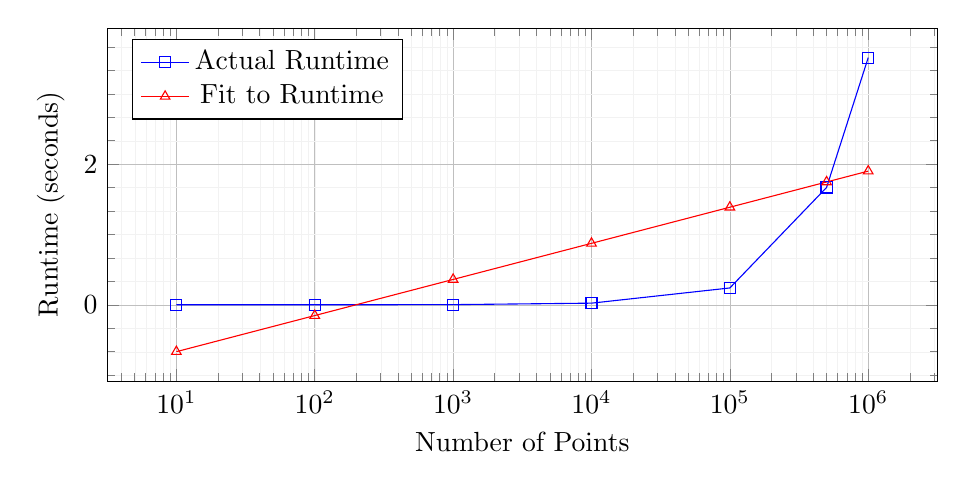
\begin{tikzpicture}
        \begin{axis}[
            xlabel={Number of Points},
            ylabel={Runtime (seconds)},
            xmode=log,
            ymode=linear,
            legend pos=north west,
            grid=both,
            grid style={line width=.1pt, draw=gray!10},
            major grid style={line width=.2pt,draw=gray!50},
            minor tick num=5,
            width=\textwidth,
            height=0.5\textwidth,
            log basis x={10},
            log basis y={10}
        ]
        \addplot[
            color=blue,
            mark=square,
            ]
            coordinates {
            (10,0.00003)
            (100,0.00021)
            (1000,0.00244)
            (10000,0.02342)
            (100000,0.23958)
            (500000,1.66867)
            (1000000,3.51449)
            };
        \addlegendentry{Actual Runtime}
        
        \addplot[
            color=red,
            mark=triangle,
            ]
            coordinates {
            (10,-0.66642)
            (100,-0.15295)
            (1000,0.36053)
            (10000,0.87401)
            (100000,1.38748)
            (500000,1.74639)
            (1000000,1.90096)
            };
        \addlegendentry{Fit to Runtime}
        
        \end{axis}
    \end{tikzpicture}
    \caption{Comparison of Empirical and Logarithmic Fit Runtime of \texttt{compute\_hull()}}
    \label{fig:runtime_graph}
\end{figure}

\section{Discussion}
The empirical runtime of the \texttt{compute\_hull()} function was
compared to the theoretical time complexity of $O(n \log n)$ using
a logarithmic regression model. The acutal runtime appears to be 
slightly slower than the theoretical $O(n \log n)$ time complexity, 
but much faster than a $O(n^2)$ fit. 


\section{Example Datasets}
\begin{figure}[h]
    \centering
    \includegraphics[width=0.6\textwidth]{100 points.png}
    \caption{Convex Hull for 100 Points}
    \label{fig:100_points}
\end{figure}

\begin{figure}[h]
    \centering
    \includegraphics[width=0.6\textwidth]{1000 points.png}
    \caption{Convex Hull for 1000 Points}
    \label{fig:1000_points}
\end{figure}

\end{document}